% GENERATED by haipipe-display scripts/build_preview.py: page 1 the display, pages 2+ how it was made. Rerun it.
\documentclass[12pt]{article}
\usepackage[letterpaper,margin=1in]{geometry}
\usepackage{fontspec}
\IfFontExistsTF{TeX Gyre Termes}{\setmainfont{TeX Gyre Termes}}{\IfFontExistsTF{Times New Roman}{\setmainfont{Times New Roman}}{}}
\usepackage{microtype}
\usepackage{graphicx,booktabs,tabularx,multirow,array,longtable,amsmath,amssymb,setspace,caption,float,xcolor}
\usepackage{fancyhdr}
\onehalfspacing
\setlength{\parindent}{0.25in}
\setlength{\parskip}{0.35em}
\pagestyle{fancy}\fancyhf{}
\renewcommand{\headrulewidth}{0pt}
\fancyfoot[C]{\thepage}
\usepackage{float}
\begin{document}
\makeatletter\renewcommand{\fps@figure}{H}\renewcommand{\fps@table}{H}\makeatother
\renewcommand{\figurename}{eFigure}\renewcommand{\tablename}{eTable}\renewcommand{\thefigure}{2}\renewcommand{\thetable}{2}
\begin{figure}
  \centering
  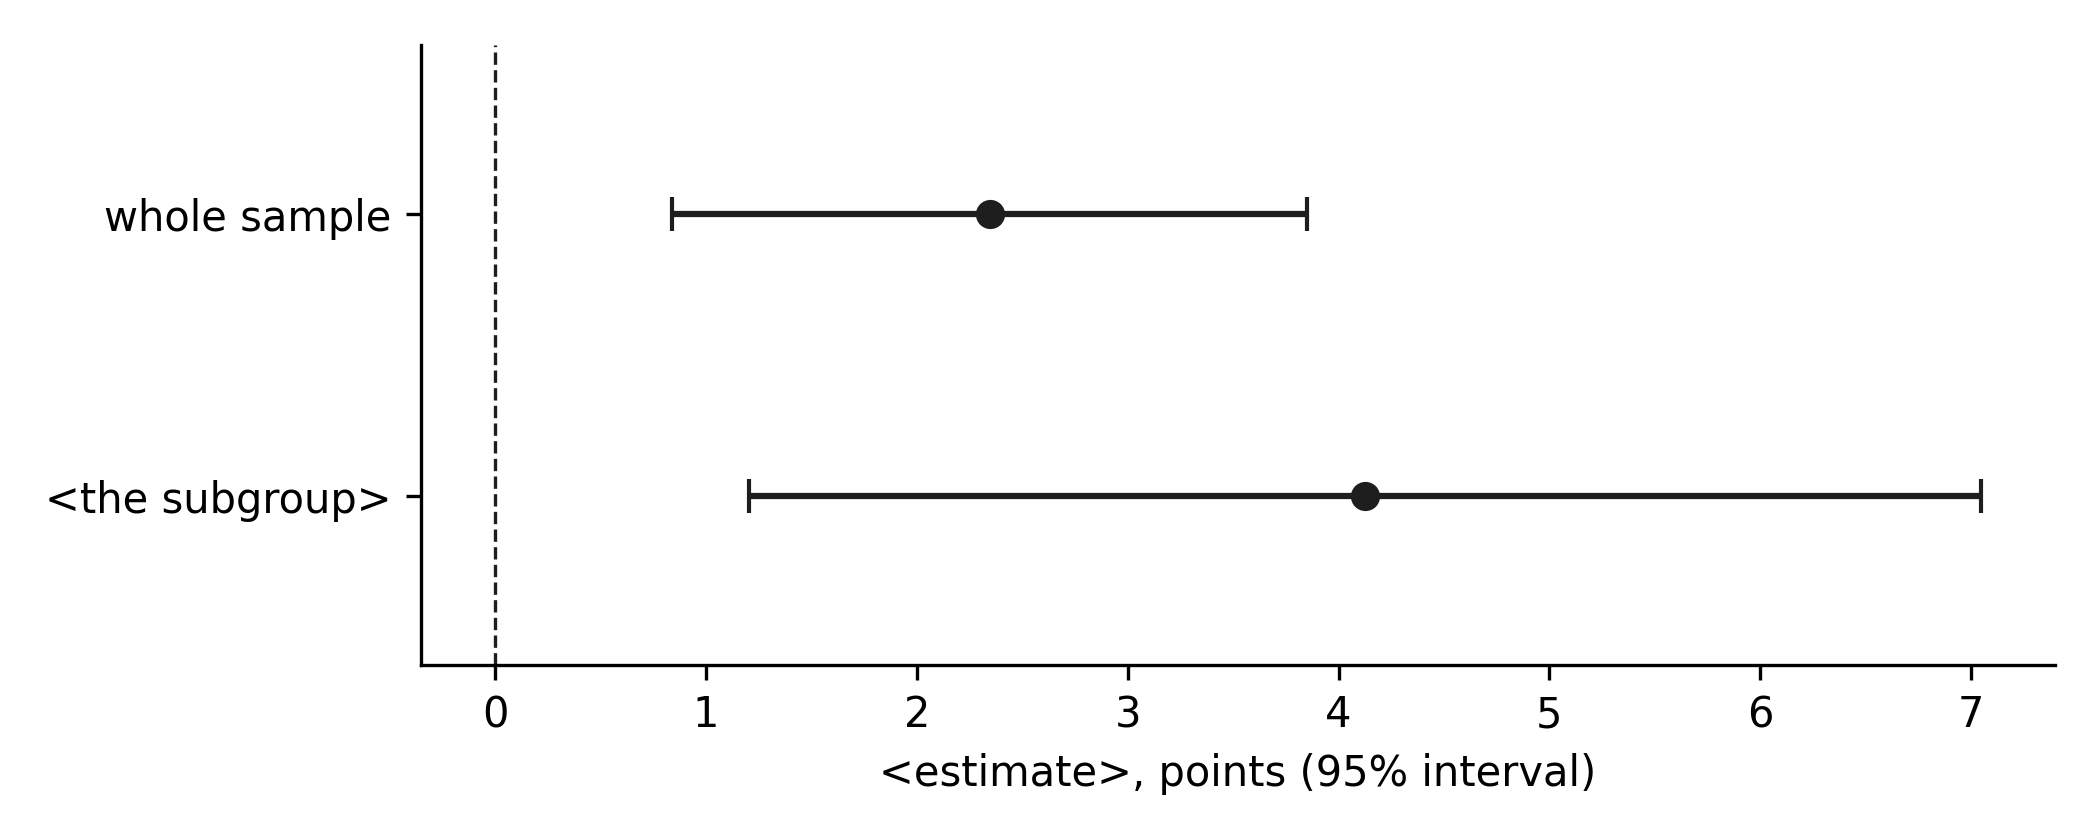
\includegraphics[width=\linewidth]{assets/figure.png}
  \caption{\textbf{<Subgroup> estimate beside the whole sample.} Each point is the same model's estimate with its 95\% interval, in everyone and in <the subgroup>; the dashed line marks zero. Placeholder figure of Tools' Paper-Example; no real data.}
  \label{fig:subgroup}
\end{figure}

\clearpage
\section*{What this display says}
In <the subgroup> the association with <the policy> is larger than in the whole sample, and its interval is wider, so the paper's answer to RQ2, for whom it changes, rests on fewer units.

\section*{How this display was made}
\subsection*{Data}
<The data source>, years <YYYY to YYYY>: the work Runs b90.j02.t01.r01 and b90.j02.t02.r01, each its result/values.csv (placeholder).

\subsection*{Sample}
\begin{itemize}\item the whole sample, 12480 units, as in Display A
\item <the subgroup>, 3120 units
\end{itemize}
\subsection*{Method}
The main model, fitted once in everyone and once in <the subgroup>; each estimate with its 95\% interval.

\subsection*{Made by}
\begin{itemize}\item \texttt{r01\_example\_main/result/values.csv} (main.b, main.ci\_lo, main.ci\_hi, sample.n\_units), the Run of \texttt{work/b90\_example\_paper\_results/j02\_example\_estimates/t01\_example\_main/}
\item \texttt{r01\_example\_subgroup/result/values.csv} (sub.b, sub.ci\_lo, sub.ci\_hi, sub.n\_units), the Run of \texttt{work/b90\_example\_paper\_results/j02\_example\_estimates/t02\_example\_subgroup/}
\item \texttt{scripts/draw\_subgroup\_estimate.py}, the worker of \texttt{t51\_display-d-subgroup-estimate/}
\end{itemize}
\subsection*{Numbers}
Every point and interval is read from the two values.csv files above; nothing is typed in.

\end{document}
